%%
% Copyright (c) 2017 - 2019, Pascal Wagler;  
% Copyright (c) 2014 - 2019, John MacFarlane
% 
% All rights reserved.
% 
% Redistribution and use in source and binary forms, with or without 
% modification, are permitted provided that the following conditions 
% are met:
% 
% - Redistributions of source code must retain the above copyright 
% notice, this list of conditions and the following disclaimer.
% 
% - Redistributions in binary form must reproduce the above copyright 
% notice, this list of conditions and the following disclaimer in the 
% documentation and/or other materials provided with the distribution.
% 
% - Neither the name of John MacFarlane nor the names of other 
% contributors may be used to endorse or promote products derived 
% from this software without specific prior written permission.
% 
% THIS SOFTWARE IS PROVIDED BY THE COPYRIGHT HOLDERS AND CONTRIBUTORS 
% "AS IS" AND ANY EXPRESS OR IMPLIED WARRANTIES, INCLUDING, BUT NOT 
% LIMITED TO, THE IMPLIED WARRANTIES OF MERCHANTABILITY AND FITNESS 
% FOR A PARTICULAR PURPOSE ARE DISCLAIMED. IN NO EVENT SHALL THE 
% COPYRIGHT OWNER OR CONTRIBUTORS BE LIABLE FOR ANY DIRECT, INDIRECT, 
% INCIDENTAL, SPECIAL, EXEMPLARY, OR CONSEQUENTIAL DAMAGES (INCLUDING,
% BUT NOT LIMITED TO, PROCUREMENT OF SUBSTITUTE GOODS OR SERVICES; 
% LOSS OF USE, DATA, OR PROFITS; OR BUSINESS INTERRUPTION) HOWEVER 
% CAUSED AND ON ANY THEORY OF LIABILITY, WHETHER IN CONTRACT, STRICT 
% LIABILITY, OR TORT (INCLUDING NEGLIGENCE OR OTHERWISE) ARISING IN 
% ANY WAY OUT OF THE USE OF THIS SOFTWARE, EVEN IF ADVISED OF THE 
% POSSIBILITY OF SUCH DAMAGE.
%%

%%
% This is the Eisvogel pandoc LaTeX template.
%
% For usage information and examples visit the official GitHub page:
% https://github.com/Wandmalfarbe/pandoc-latex-template
%%

\PassOptionsToPackage{unicode=true}{hyperref} % options for packages loaded elsewhere
\PassOptionsToPackage{hyphens}{url}
\PassOptionsToPackage{dvipsnames,svgnames*,x11names*,table}{xcolor}
%
\documentclass[
  10pt,
  english,
  letterpaper,
,tablecaptionabove
]{scrartcl}
\usepackage{lmodern}
\usepackage{setspace}
\setstretch{1.2}
\usepackage{amssymb,amsmath}
\usepackage{ifxetex,ifluatex}
\ifnum 0\ifxetex 1\fi\ifluatex 1\fi=0 % if pdftex
  \usepackage[T1]{fontenc}
  \usepackage[utf8]{inputenc}
  \usepackage{textcomp} % provides euro and other symbols
\else % if luatex or xelatex
  \usepackage{unicode-math}
  \defaultfontfeatures{Scale=MatchLowercase}
  \defaultfontfeatures[\rmfamily]{Ligatures=TeX,Scale=1}
\fi
% use upquote if available, for straight quotes in verbatim environments
\IfFileExists{upquote.sty}{\usepackage{upquote}}{}
\IfFileExists{microtype.sty}{% use microtype if available
  \usepackage[]{microtype}
  \UseMicrotypeSet[protrusion]{basicmath} % disable protrusion for tt fonts
}{}
\makeatletter
\@ifundefined{KOMAClassName}{% if non-KOMA class
  \IfFileExists{parskip.sty}{%
    \usepackage{parskip}
  }{% else
    \setlength{\parindent}{0pt}
    \setlength{\parskip}{6pt plus 2pt minus 1pt}}
}{% if KOMA class
  \KOMAoptions{parskip=half}}
\makeatother
\usepackage{xcolor}
\definecolor{default-linkcolor}{HTML}{A50000}
\definecolor{default-filecolor}{HTML}{A50000}
\definecolor{default-citecolor}{HTML}{4077C0}
\definecolor{default-urlcolor}{HTML}{4077C0}
\IfFileExists{xurl.sty}{\usepackage{xurl}}{} % add URL line breaks if available
\IfFileExists{bookmark.sty}{\usepackage{bookmark}}{\usepackage{hyperref}}
\hypersetup{
  pdftitle={AVL Trees (Part 2)},
  pdfauthor={Connor Baker},
  pdfsubject={AVL Trees},
  pdfkeywords={Lecture, AVL, Self-Balancing Trees},
  pdfborder={0 0 0},
  breaklinks=true}
\urlstyle{same}  % don't use monospace font for urls
\usepackage[margin=2.5cm,includehead=true,includefoot=true,centering]{geometry}
\usepackage{listings}
\newcommand{\passthrough}[1]{#1}
\lstset{defaultdialect=[5.3]Lua}
\lstset{defaultdialect=[x86masm]Assembler}
\usepackage{graphicx,grffile}
\makeatletter
\def\maxwidth{\ifdim\Gin@nat@width>\linewidth\linewidth\else\Gin@nat@width\fi}
\def\maxheight{\ifdim\Gin@nat@height>\textheight\textheight\else\Gin@nat@height\fi}
\makeatother
% Scale images if necessary, so that they will not overflow the page
% margins by default, and it is still possible to overwrite the defaults
% using explicit options in \includegraphics[width, height, ...]{}
\setkeys{Gin}{width=\maxwidth,height=\maxheight,keepaspectratio}
\setlength{\emergencystretch}{3em}  % prevent overfull lines
\providecommand{\tightlist}{%
  \setlength{\itemsep}{0pt}\setlength{\parskip}{0pt}}
\setcounter{secnumdepth}{-\maxdimen} % remove section numbering
% Redefines (sub)paragraphs to behave more like sections
\ifx\paragraph\undefined\else
  \let\oldparagraph\paragraph
  \renewcommand{\paragraph}[1]{\oldparagraph{#1}\mbox{}}
\fi
\ifx\subparagraph\undefined\else
  \let\oldsubparagraph\subparagraph
  \renewcommand{\subparagraph}[1]{\oldsubparagraph{#1}\mbox{}}
\fi

% Make use of float-package and set default placement for figures to H
\usepackage{float}
\floatplacement{figure}{H}

\setcounter{page}{0}
\lstset{breaklines=true}
\lstset{postbreak=\raisebox{0ex}[0ex][0ex]{\ensuremath{\color{blue}\hookrightarrow\space}}}
\usepackage{datetime}
\settimeformat{ampmtime}
\usepackage{lastpage}
\ifnum 0\ifxetex 1\fi=0 % if pdftex or luatex
  \usepackage[shorthands=off,main=english]{babel}
\else % if xetex
    % See issue https://github.com/reutenauer/polyglossia/issues/127
  \renewcommand*\familydefault{\sfdefault}
    % load polyglossia as late as possible as it *could* call bidi if RTL lang (e.g. Hebrew or Arabic)
  \usepackage{polyglossia}
  \setmainlanguage[]{english}
\fi

\title{AVL Trees (Part 2)}
\usepackage{etoolbox}
\makeatletter
\providecommand{\subtitle}[1]{% add subtitle to \maketitle
  \apptocmd{\@title}{\par {\large #1 \par}}{}{}
}
\makeatother
\subtitle{AVL Tree Balancing}
\author{Connor Baker}
\date{2019-04-11, Compiled on \today~at \currenttime}





%%
%% added
%%

%
% language specification
%
% If no language is specified, use English as the default main document language.
%


%
% for the background color of the title page
%
\usepackage{pagecolor}
\usepackage{afterpage}

%
% TOC depth and 
% section numbering depth
%
\setcounter{tocdepth}{3}

%
% break urls
%
\PassOptionsToPackage{hyphens}{url}

%
% When using babel or polyglossia with biblatex, loading csquotes is recommended 
% to ensure that quoted texts are typeset according to the rules of your main language.
%
\usepackage{csquotes}

%
% captions
%
\definecolor{caption-color}{HTML}{777777}
\usepackage[font={stretch=1.2}, textfont={color=caption-color}, position=top, skip=4mm, labelfont=bf, singlelinecheck=false, justification=raggedright]{caption}
\setcapindent{0em}

%
% blockquote
%
\definecolor{blockquote-border}{RGB}{221,221,221}
\definecolor{blockquote-text}{RGB}{119,119,119}
\usepackage{mdframed}
\newmdenv[rightline=false,bottomline=false,topline=false,linewidth=3pt,linecolor=blockquote-border,skipabove=\parskip]{customblockquote}
\renewenvironment{quote}{\begin{customblockquote}\list{}{\rightmargin=0em\leftmargin=0em}%
\item\relax\color{blockquote-text}\ignorespaces}{\unskip\unskip\endlist\end{customblockquote}}

%
% Source Sans Pro as the de­fault font fam­ily
% Source Code Pro for monospace text
%
% 'default' option sets the default 
% font family to Source Sans Pro, not \sfdefault.
%
\usepackage[default]{sourcesanspro}
\usepackage{sourcecodepro}

% XeLaTeX specific adjustments for straight quotes: https://tex.stackexchange.com/a/354887
% This issue is already fixed (see https://github.com/silkeh/latex-sourcecodepro/pull/5) but the 
% fix is still unreleased.
% TODO: Remove this workaround when the new version of sourcecodepro is released on CTAN.
\ifxetex
\makeatletter
\defaultfontfeatures[\ttfamily]
  { Numbers   = \sourcecodepro@figurestyle,
    Scale     = \SourceCodePro@scale,
    Extension = .otf }
\setmonofont
  [ UprightFont    = *-\sourcecodepro@regstyle,
    ItalicFont     = *-\sourcecodepro@regstyle It,
    BoldFont       = *-\sourcecodepro@boldstyle,
    BoldItalicFont = *-\sourcecodepro@boldstyle It ]
  {SourceCodePro}
\makeatother
\fi

%
% heading color
%
\definecolor{heading-color}{RGB}{40,40,40}
\addtokomafont{section}{\color{heading-color}}
% When using the classes report, scrreprt, book, 
% scrbook or memoir, uncomment the following line.
%\addtokomafont{chapter}{\color{heading-color}}

%
% variables for title and author
%
\usepackage{titling}
\title{AVL Trees (Part 2)}
\author{Connor Baker}

%
% tables
%

%
% remove paragraph indention
%
\setlength{\parindent}{0pt}
\setlength{\parskip}{6pt plus 2pt minus 1pt}
\setlength{\emergencystretch}{3em}  % prevent overfull lines

%
%
% Listings
%
%


%
% listing colors
%
\definecolor{listing-background}{HTML}{F7F7F7}
\definecolor{listing-rule}{HTML}{B3B2B3}
\definecolor{listing-numbers}{HTML}{B3B2B3}
\definecolor{listing-text-color}{HTML}{000000}
\definecolor{listing-keyword}{HTML}{435489}
\definecolor{listing-identifier}{HTML}{435489}
\definecolor{listing-string}{HTML}{00999A}
\definecolor{listing-comment}{HTML}{8E8E8E}
\definecolor{listing-javadoc-comment}{HTML}{006CA9}

\lstdefinestyle{eisvogel_listing_style}{
  language         = java,
  numbers          = left,
  xleftmargin      = 2.7em,
  framexleftmargin = 2.5em,
  backgroundcolor  = \color{listing-background},
  basicstyle       = \color{listing-text-color}\small\ttfamily{}\linespread{1.15}, % print whole listing small
  breaklines       = true,
  frame            = single,
  framesep         = 0.19em,
  rulecolor        = \color{listing-rule},
  frameround       = ffff,
  tabsize          = 4,
  numberstyle      = \color{listing-numbers},
  aboveskip        = -0.7em,
  belowskip        = 0.1em,
  abovecaptionskip = 0em,
  belowcaptionskip = 1em,
  keywordstyle     = \color{listing-keyword}\bfseries,
  classoffset      = 0,
  sensitive        = true,
  identifierstyle  = \color{listing-identifier},
  commentstyle     = \color{listing-comment},
  morecomment      = [s][\color{listing-javadoc-comment}]{/**}{*/},
  stringstyle      = \color{listing-string},
  showstringspaces = false,
  escapeinside     = {/*@}{@*/}, % Allow LaTeX inside these special comments
  literate         =
  {á}{{\'a}}1 {é}{{\'e}}1 {í}{{\'i}}1 {ó}{{\'o}}1 {ú}{{\'u}}1
  {Á}{{\'A}}1 {É}{{\'E}}1 {Í}{{\'I}}1 {Ó}{{\'O}}1 {Ú}{{\'U}}1
  {à}{{\`a}}1 {è}{{\'e}}1 {ì}{{\`i}}1 {ò}{{\`o}}1 {ù}{{\`u}}1
  {À}{{\`A}}1 {È}{{\'E}}1 {Ì}{{\`I}}1 {Ò}{{\`O}}1 {Ù}{{\`U}}1
  {ä}{{\"a}}1 {ë}{{\"e}}1 {ï}{{\"i}}1 {ö}{{\"o}}1 {ü}{{\"u}}1
  {Ä}{{\"A}}1 {Ë}{{\"E}}1 {Ï}{{\"I}}1 {Ö}{{\"O}}1 {Ü}{{\"U}}1
  {â}{{\^a}}1 {ê}{{\^e}}1 {î}{{\^i}}1 {ô}{{\^o}}1 {û}{{\^u}}1
  {Â}{{\^A}}1 {Ê}{{\^E}}1 {Î}{{\^I}}1 {Ô}{{\^O}}1 {Û}{{\^U}}1
  {œ}{{\oe}}1 {Œ}{{\OE}}1 {æ}{{\ae}}1 {Æ}{{\AE}}1 {ß}{{\ss}}1
  {ç}{{\c c}}1 {Ç}{{\c C}}1 {ø}{{\o}}1 {å}{{\r a}}1 {Å}{{\r A}}1
  {€}{{\EUR}}1 {£}{{\pounds}}1 {«}{{\guillemotleft}}1
  {»}{{\guillemotright}}1 {ñ}{{\~n}}1 {Ñ}{{\~N}}1 {¿}{{?`}}1
  {…}{{\ldots}}1 {≥}{{>=}}1 {≤}{{<=}}1 {„}{{\glqq}}1 {“}{{\grqq}}1
  {”}{{''}}1
}
\lstset{style=eisvogel_listing_style}

\lstdefinelanguage{XML}{
  morestring      = [b]",
  moredelim       = [s][\bfseries\color{listing-keyword}]{<}{\ },
  moredelim       = [s][\bfseries\color{listing-keyword}]{</}{>},
  moredelim       = [l][\bfseries\color{listing-keyword}]{/>},
  moredelim       = [l][\bfseries\color{listing-keyword}]{>},
  morecomment     = [s]{<?}{?>},
  morecomment     = [s]{<!--}{-->},
  commentstyle    = \color{listing-comment},
  stringstyle     = \color{listing-string},
  identifierstyle = \color{listing-identifier}
}

%
% header and footer
%
\usepackage{fancyhdr}

\fancypagestyle{eisvogel-header-footer}{
  \fancyhead{}
  \fancyfoot{}
  \lhead[2019-04-11]{AVL Trees (Part 2)}
  \chead[]{}
  \rhead[AVL Trees (Part 2)]{2019-04-11}
  \lfoot[\thepage~of \pageref{LastPage}]{Connor Baker}
  \cfoot[]{}
  \rfoot[Connor Baker]{\thepage~of \pageref{LastPage}}
  \renewcommand{\headrulewidth}{0.4pt}
  \renewcommand{\footrulewidth}{0.4pt}
}
\pagestyle{eisvogel-header-footer}

%%
%% end added
%%

\begin{document}

%%
%% begin titlepage
%%

\begin{titlepage}
\newgeometry{left=6cm}
\definecolor{titlepage-color}{HTML}{FFFFFF}
\newpagecolor{titlepage-color}\afterpage{\restorepagecolor}
\newcommand{\colorRule}[3][black]{\textcolor[HTML]{#1}{\rule{#2}{#3}}}
\begin{flushleft}
\noindent
\\[-1em]
\color[HTML]{0d47a1}
\makebox[0pt][l]{\colorRule[0d47a1]{1.3\textwidth}{2pt}}
\par
\noindent

{ \setstretch{1.4}
\vfill
\noindent {\huge \textbf{\textsf{AVL Trees (Part 2)}}}
\vskip 1em
{\Large \textsf{AVL Tree Balancing}}
\vskip 2em
\noindent
{\Large \textsf{Connor Baker}
\vfill
}


\textsf{2019-04-11, Compiled on \today~at \currenttime}}
\end{flushleft}
\end{titlepage}
\restoregeometry

%%
%% end titlepage
%%



\hypertarget{avl-trees-part-2}{%
\section{AVL Trees (Part 2)}\label{avl-trees-part-2}}

\hypertarget{review-avl-trees}{%
\subsection{Review: AVL Trees}\label{review-avl-trees}}

\begin{itemize}
\tightlist
\item
  Binary search tree with balance property
\item
  Re-balancing might be triggered by insertion into or removal from the
  tree

  \begin{itemize}
  \tightlist
  \item
    Check the height of the left and right sub-trees and keep the
    difference bounded by 1
  \item
    Might require a single or a double rotation
  \end{itemize}
\end{itemize}

\hypertarget{avl-tree-balance-cases}{%
\subsection{AVL Tree Balance Cases}\label{avl-tree-balance-cases}}

\begin{itemize}
\tightlist
\item
  Height imbalance means some node \passthrough{\lstinline!n!} whose two
  sub-trees differ by two

  \begin{itemize}
  \tightlist
  \item
    Case 1: Insertion into the left subtree of the left child or
    \passthrough{\lstinline!n!}
  \item
    Case 2: Insertion into the right subtree of the left child or
    \passthrough{\lstinline!n!}
  \item
    Case 3: Insertion into the left subtree of the right child or
    \passthrough{\lstinline!n!}
  \item
    Case 4: Insertion into the right subtree of the right child or
    \passthrough{\lstinline!n!}
  \end{itemize}
\item
  Note the symmetry between cases 1 and four and cases 2 and 3

  \begin{itemize}
  \tightlist
  \item
    Cases 1 and 4 take place on the outside of the tree and require only
    a single rotation
  \item
    Cases 2 and 3 take place inside the tree and require a double
    rotation
  \end{itemize}
\item
  Similar cases when a deleiton causes an imbalance
\end{itemize}

\hypertarget{case-examples}{%
\subsection{Case Examples}\label{case-examples}}

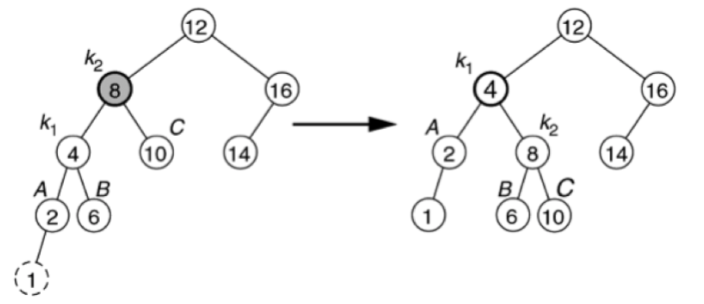
\includegraphics[width=0.5\textwidth,height=\textheight]{images/1.png}
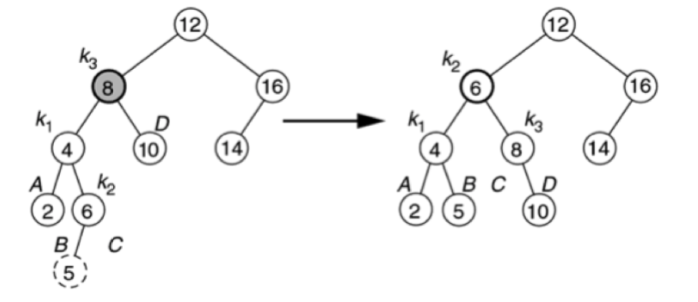
\includegraphics[width=0.5\textwidth,height=\textheight]{images/2.png}

\hypertarget{left-right-rotation-code}{%
\subsection{Left-Right Rotation Code}\label{left-right-rotation-code}}

The following code comes from our book by Weiss, Figures 19.24, 19.27,
19.32, and 19.33.

\begin{lstlisting}[language=Java]
/**
 * Rotate binary tree node with left chid.
 * For AVL trees, this is a single rotation for case 1.
 */
static BinaryNode rotateWithLeftChild( BinaryNode k2 ){
  BinaryNode k1 = k2.left;
  k2.left = k1.right;
  k1.right = k2;
  return k1;
}

/**
 * Rotate binary tree node with right child.
 * For AVL trees, this is a single rotation for case 4.
 */
static BinaryNode rotateWithRightChild( BinaryNode k1 ) {
  BinaryNode k2 = k1.right;
  k1.right = k2.left;
  k2.left = k1;
  return k2;
}

 /**
  * Double rotate binary tree node: first left child
  * with its right child; then node k3 with new left child.
  * For AVL trees, this is a double rotation for case 2.
  */
static BinaryNode doubleRotateWithLeftChild( BinaryNode k3 ) {
  k3.left = rotateWithRightChild( k3.left );
  return rotateWithLeftChild( k3 );
}

 /**
  * Double rotate binary tree node: first right child
  * with its left child; then node k3 with new right child.
  * For AVL trees, this is a double rotation for case 3.
  */
static BinaryNode doubleRotateWithRightChild( BinaryNode k1 ) {
  k1.left = rotateWithLeftChild( k1.right );
  return rotateWithRightChild( k1 );
}
\end{lstlisting}

\begin{itemize}
\tightlist
\item
  What's our complexity?

  \begin{itemize}
  \tightlist
  \item
    Each method is \(O(1)\) and even with composition the result is
    still \(O(1)\)
  \end{itemize}
\end{itemize}

\hypertarget{practice}{%
\subsection{Practice}\label{practice}}

\begin{figure}
\centering
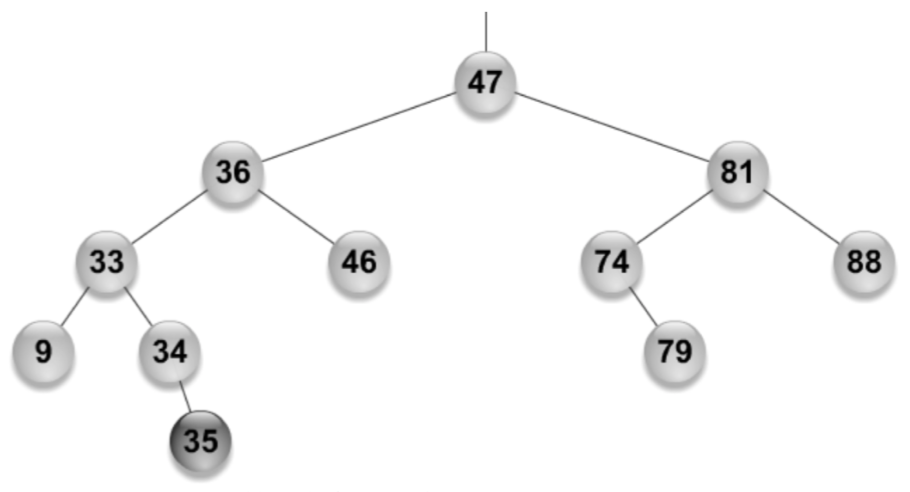
\includegraphics[width=0.5\textwidth,height=\textheight]{images/3.png}
\caption{An unbalanced AVL tree}
\end{figure}

\begin{itemize}
\tightlist
\item
  Assume that we just inserted 35 into the above tree
\item
  Which node(s) do we need to re-balance?

  \begin{itemize}
  \tightlist
  \item
    \textbf{ANSWER}
  \end{itemize}
\item
  How do we re-balance them?

  \begin{itemize}
  \tightlist
  \item
    \textbf{ANSWER}
  \end{itemize}
\end{itemize}

\hypertarget{excerpt-of-insertion-code}{%
\subsection{Excerpt of Insertion Code}\label{excerpt-of-insertion-code}}

\textbf{Use method names that are equivalent to the above methods taken
from the textbook}

\begin{lstlisting}[language=Java]
private AvlNode insert( Comparable x, AvlNode t ) {
  // Insertion
  if (t == null) {
    // Found the spot to insert; return new node with data
    t = new AvlNode( x, null, null );
  } else if ( x.compareTo( t.element ) < 0) {
    // Head to left recursively
    t.left = insert( x, t.left );
  } else {
    // Head to right recursively
    t.right = insert( x, t.right );
  }

  // Check balance and rotate
  if (height(t.left) - height(t.right) == 2) {
    // Left subtree is deeper than right subtree
    if (height(t.left.left) > t.left.right) {
      // Outer tree unbalanced; single rotation
      t = rightRotate( t );
    } else {
      // the inserted node went left-right; double rotation
      t = leftRightRotate( t );
    }
  } else {
    // Symmetric cases for the right subtree being deeper than the left
  }

  // Return the new root
  return t;
}
\end{lstlisting}

\hypertarget{avl-deletion}{%
\subsection{AVL Deletion}\label{avl-deletion}}

\begin{itemize}
\tightlist
\item
  Start with our normal BST deletion

  \begin{itemize}
  \tightlist
  \item
    0 children (node is a leaf): delete the node
  \item
    1 child: delete the node and connect the child to the parent
  \item
    2 children: put the predecessor/successor to replace the node, then
    delete the predecessor/successor
  \end{itemize}
\item
  Which nodes should we check for an imbalance?

  \begin{itemize}
  \tightlist
  \item
    0 children / 1 child: all nodes on the path from the deleted node to
    the root
  \item
    2 children: all nodes on the path from the deleted
    predecessor/successsor to the root
  \end{itemize}
\end{itemize}

\hypertarget{avl-deletion-imbalance-cases}{%
\subsection{AVL Deletion Imbalance
Cases}\label{avl-deletion-imbalance-cases}}

\begin{itemize}
\tightlist
\item
  \passthrough{\lstinline!n!} is the node with the imbalanced heights

  \begin{itemize}
  \tightlist
  \item
    Deleting from the right subtree of \passthrough{\lstinline!n!}

    \begin{itemize}
    \tightlist
    \item
      The left subtree of a left child is too tall: outside case, single
      rotation
    \item
      The right subtree of a left child is too tall: inside case, double
      rotation
    \item
      Both subtrees of the left child are too tall: same as the first
      case
    \end{itemize}
  \item
    Symmetric cases for deleting from the left side

    \begin{itemize}
    \tightlist
    \item
      Right subtree of a right child is too tall: outside case, single
      rotation
    \item
      Left subtree of a right child is too tall: inside case, double
      rotation
    \item
      Both subtrees of a right child are too tall: same as the first
      case
    \end{itemize}
  \end{itemize}
\end{itemize}

\hypertarget{complexity}{%
\subsection{Complexity}\label{complexity}}

\textbf{Proposition}: maintaining the AVL balance property during
insertion and removal will yield a tree with \(N\) N nodes and height
\(O(\log(N))\)

\textbf{Theorem 19.3}: An AVL tree of height \(H\) has at least
\(H_{H+3} - 1\) where \(F_i\) is the \(i\)th Fibonacci number

\textbf{Proof}: Let \(S_H\) be the size of the smallest AVL tree of
height \(H\). Clearly, \(S_0 = 1\) and \(S_1 = 2\). The smallest AVL
tree of height \(H\) must have subtrees of height \(H – 1\) and
\(H – 2\). The reason is that at least one subtree has height \(H – 1\)
and the balance condition implies that subtree heights can differ by at
most \(1\). These subtrees must themselves have the fewest number of
nodes for their heights, so \(S_H = S_H – 1 + S_H – 2 + 1\). The proof
can be completed by using an induction argument.

\emph{Corollary}: We know that
\(F_i \approx \frac{\varphi^i}{\sqrt{5}}\) where \(F_i\) is the \(i\)th
Fibonacci number and \(\varphi = \frac{1+\sqrt{5}}{2} \approx 1.618\).
Then with an AVL tree of height \(H\) we have at least
\(\frac{\varphi^{H+3}}{\sqrt{5}}\) nodes, and its depth is at most
logarithmic. The height of an AVL tree satisfies

\[H < 1.44 \log(N+2) - 1.328.\]

Therefore the worst-case height is at most roughly \(44\%\) more than
the minimum possible for binary trees.

\emph{Corollary}: All searching operations in an AVL tree have
logarithmic worst-case bounds.

\emph{Note}: The depth of an average node in a randomly constructed AVL
tree tends to be very close to \(\log(N)\). The exact answer has not yet
been established analytically. We do not even know whether the form is
\(\log(N) + C\) or \((1 + \epsilon) \log(N) + C\), for some \(\epsilon\)
that would be approximately \(0.01\). Simulations have been unable to
demonstrate convincingly that one form is more plausible than the other.

\hypertarget{rotation-overhead}{%
\subsection{Rotation Overhead}\label{rotation-overhead}}

\begin{itemize}
\tightlist
\item
  Single rotation / double rotation once

  \begin{itemize}
  \tightlist
  \item
    \(O(1)\) complexity
  \end{itemize}
\item
  How many rotations are needed for

  \begin{itemize}
  \tightlist
  \item
    Insertion: 2 (worst-case double rotation), which is \(O(1)\)
  \item
    Removal: 2 (worst-case double rotation), which is \(O(1)\)
  \end{itemize}
\item
  Overall complexity

  \begin{itemize}
  \tightlist
  \item
    Bounded by \(O(\)height\() = O(\log_2(N)\)
  \end{itemize}
\end{itemize}

\hypertarget{next-lecture}{%
\subsection{Next Lecture}\label{next-lecture}}

\begin{itemize}
\tightlist
\item
  Topic: more self-balancing binary search trees

  \begin{itemize}
  \tightlist
  \item
    Red-black trees
  \end{itemize}
\item
  Reading: Chapter 19.5 - 19.7
\end{itemize}

\end{document}
